\documentclass[journal=langd5,manuscript=article]{achemso}
\usepackage{lipsum}
%\usepackage[margin=1in]{geometry}
\usepackage{rotating}
\usepackage{lscape}
\usepackage[T1]{fontenc}
\usepackage[utf8]{inputenc}
\usepackage{flafter}
%\usepackage{floatflt}
\usepackage{placeins}
\usepackage{siunitx}
\usepackage{graphicx}
\graphicspath{{./figures/}}% Include figure files
%\usepackage{epstopdf}
\usepackage{dcolumn}% Align table columns on decimal point
\usepackage{appendix}
\usepackage{amsmath}
\usepackage{cases}
\usepackage{calc}
\usepackage{amssymb}
\usepackage[dvips]{color}
\usepackage{color}
\usepackage{enumitem}
\usepackage{soul}
\usepackage{indentfirst}
\usepackage{hyphenat}
\usepackage{xspace}
\usepackage{subcaption}
\usepackage{booktabs}
\usepackage{multirow}
\usepackage{tabularx}
\usepackage{xcolor}
\usepackage{lineno}
\usepackage{setspace}
\usepackage{hyperref}
\usepackage{xr-hyper} % must come after hyperref
\usepackage[nameinlink]{cleveref}

\externaldocument{supporting_information} 
\newcommand{\tbxmulticol}[3]
    {\multicolumn{#1}
                 {>{\centering\hsize=\dimexpr#1\hsize+#1\tabcolsep+\arrayrulewidth\relax}#2}
                 {#3}}
\newcommand{\ra}[1]{\renewcommand{\arraystretch}{#1}}
%\newcommand{\cmpersec}{$\frac{\text{cm}}{\text{s}}$~}
\newcommand{\cmpersec}{cm/s~}
\newcommand{\etal}{\textit{et al.}}
\newcommand{\na}{Na\textsuperscript{+}}
\newcommand{\li}{Li\textsuperscript{+}}
\newcommand{\mg}{Mg\textsuperscript{2+}}
\newcommand{\cl}{Cl\textsuperscript{-}}
\newcommand{\mgcl}{MgCl\textsubscript{2}}
\newcommand{\nacl}{NaCl}
\newcommand{\licl}{LiCl}
\newcommand{\PM}{$\pm$~}
\newcommand{\invnm}{$\text{\si{\nm}}^{-1}$~}
\newcommand{\nmeter}{\si{\nm}~}
\renewcommand{\arraystretch}{1.8}
\newcommand{\TODO}{\hl{TODO}~}
\newcommand{\about}{$\sim$}
\newcommand{\aangstroms}{{\aa}ngstr{\"o}ms}
\newcommand{\aangstrom}{{\aa}ngstr{\"o}m}
\newcommand{\sigmaij}{$\sigma_{ij}$}
\newcommand{\epsilonij}{$\epsilon_{ij}$}
\newcommand{\db}{$\text{D}_\text{B}$}
\newcommand{\dhh}{$\text{D}_\text{hh}$}
\newcommand{\dc}{$\text{2D}_\text{C}$}
\newcommand{\Vh}{$\text{V}_\text{H}$}
\newcommand{\Vc}{$\text{V}_\text{C}$}
\newcommand{\Vl}{$\text{V}_\text{L}$}
\newcommand{\al}{$\text{A}_\text{L}$}

\title{Alteration of lipid bilayer structure by \mg}
\author{Matthew Saunders}
\email{mwsaunders@usf.edu}
\affiliation{Department of Molecular Biosciences
University of South Florida, Tampa, Florida 33620}
\affiliation{Department of Physics, University of South Florida, Tampa
Florida 33620}
\author{Sagar A. Pandit}
%\email{pandit@usf.edu}
\affiliation{Department of Physics, University of South Florida, Tampa
Florida 33620}
\author{Sameer Varma}
\email{svarma@usf.edu}
\affiliation{Department of Molecular Biosciences, University of South Florida, Tampa
Florida 33620}



\date{\today}


\begin{document}
\begin{abstract}

Developing molecular mechanics force fields to model interactions of biological
membranes with \mg{} cations is challenging. There are no direct estimates of the
binding modes of \mg~ions with lipid headgroups or other phosphates in the condensed
phase. Experimental data on lipid bilayers in \mg{} solution are sparse and limited
to biologically relevant but very low ion concentrations. At these concentrations, no
statistically discernible effects on bilayer properties are observed.
Simulations at these concentrations are difficult due to system size and the extensive conformational
sampling required for force-field development.
Considering these issues, we previously calibrated \mg-lipid Lennard-Jones cross-terms
using benchmarked quantum mechanical (QM) target data on small clusters of ions and
ligands representative of common cation binding sites on 1-palmitoyl-2-
oleoyl-sn-glycero-phosphatidylcholine (POPC). Our
simulations with these new \mg{} parameters yielded bilayer structures very similar
to those without salt, in agreement with available experimental data. 
We adopted this strategy because it worked well for modeling
membrane interactions with monovalent cations, for which additional experimental
data are available. However, newer studies from our group show that for \mg~ions,
the choice of target \mg-lipid mimetic clusters is non-trivial. Inclusion of fully
coordinated (6-fold) \mg~ions, which better represent potential ion-lipid structures
in the condensed phase, may be critical for selecting models that reproduce
experimental condensed-phase interactions of \mg~with nucleotide phosphates.
Using this new protocol, we propose an additional set of \mg-lipid interaction
Lennard-Jones cross-terms. With this parameter set, we find that at concentrations 
between 100-200 mM, there is a systematic thickening of the lipid bilayer, not observed
with our previous \mg-lipid model. Additionally, compared to the earlier model, we
observe more \mg~adsorbed on the bilayer and a larger fraction directly
coordinating lipid headgroups. However, the new model does not alter our previous
observation that structural changes in the bilayer correlate with the amount of
ionic charge directly coordinating lipid molecules.

\end{abstract}

\linenumbers
\doublespacing
\section{Introduction}

Salts have a well characterized behavior at interfaces in the condensed phase -- ions form a classic double layer, where
one charge accumulates near the substrate's surface, and the second charge then accumulates to compensate for 
that charge~\cite{israelachvili:2011:intermol}.
This can be explained using a mean-field approximation. 
However, the mean-field approximation does not provide details on specific interactions between ionic species and 
interface moieties. These details are non-trivial, especially in the case of
phospholipid membranes, where the substrate itself is liquid and can adopt new conformations in response to ion adsorption. 

Molecular dynamics (MD) simulations can, in principle, provide such details. 
However, the development of MD force fields for \mg{}, and modeling their interaction with lipid bilayers poses significant challenges.
Firstly, experimental data needed for force field development and validation is scarce.
To our knowledge, there are no direct estimates on the binding modes of \mg~ions with lipid headgroups or any other phosphates in the condensed phase. 
Secondly, the effects of \mg{} on lipid bilayer structure are only known for small concentrations
of salt~\cite{kurakin:2022:cations,kurakin:2021:effect}.
Simulations such low salt concentrations push the limits of hardware requirements for conformational sampling and force field testing. 
For example, in our previous simulations with \na{}~\cite{saunders:2022}, we observed between 75-90 \na{} ions adsorbed to an equilibrated lipid bilayer of 
100 POPC molecules per leaflet. If we assume similar numbers of \mg to be adsorbed, 
simulating at a biologically relevant concentration of 0.5 mM~\cite{romani:1992:regulation} will require more than 11 million waters.
Additionally, since the residence time of waters in the first shell of \mg~is 
of the order of a microsecond \cite{neely:1970,Palinkas:1982,bleuzen:1997}, 
capturing statistics on water-lipid exchanges in the first shell of \mg~requires prohibitively long MD simulations. 

Considering these issues, we previously chose to calibrate \mg-lipid Lennard-Jones (LJ) terms using 
benchmarked quantum mechanical (QM) target data clusters of small molecules representative of the
ion binding sites on 1-palmitoyl-2-oleoyl-sn-glycero-phosphatidylcholine (POPC)~\cite{saunders:2022}. 
Methyl acetate (MeAc) and diethyl phosphate (DEPh) were taken as small molecule representatives for lipid headgroups, 
and we targeted the changes in energy and structure associated with replacing water molecules in \mg-water clusters with these smaller molecules.  
Using this model we found that at about 100 mM concentration, \mg adsorbed into the headgroup region of POPC bilayer, 
but without losing its inner-shell waters (steric binding mode). We also observed formation of ion double layer at the headgroup-water interface.
However, \mg~adsorption had a negligible effect on POPC bilayer structure. We posited that since our model at 
high salt did not affect bilayer structure, our model at low experimental salt concentration will also not affect POPC bilayer structure; making the result consistent with experiment. 
We adopted this strategy because we showed that it worked well for modeling interactions of lipid bilayers with monovalent cations \cite{saunders:2022}. Prior to our development, all simulations, irrespective of the employed force field, reported that monovalent salts thickened POPC bilayers \cite{sachs:2004,melcr:2018,jurkiewicz:2012,kruczek:2017}. 
In contrast, experiments reported insignificant changes in POPC lipid bilayer structure \cite{pabst:2007:rigidification,petrache:2006:swelling}. 
The use of our new \na-lipid LJ terms resolved this discrepancy to a large extent \cite{saunders:2022}. 
Recent developments in our lab, however, motivate us to explore a modified strategy for developing \mg-lipid LJ terms. 
Our recent work of polarizable force fields for describing \mg-protein/nucleotide interactions \cite{julian:2023:mg} suggests that perhaps within the classical framework, a single set of force field parameters for \mg do not perform well at simultaneously reproducing 
energies of both fully coordinated (6-fold)
and partially coordinated \mg~structures. 
Furthermore, force field developed using 6-fold coordinated structures performed excellently at reproducing not only local interactions of 
\mg~ions in clusters containing nucleotide phosphates but also condensed phase binding free energies of \mg~ions with nucleotides \cite{julian:2023:mg}. We have shown that this strategy also works for other cations \cite{JACS2025} 
Fully coordinated 6-fold clusters of \mg~were not considered in the development of our previous \mg{} model~\cite{saunders:2024}, in which target data consisted of only partially coordinated structures of \mg.

Here we apply this new protocol to develop a new set of \mg{}-lipid LJ
terms. Our target data consists exclusively of full 6-fold coordinated \mg~clusters with 
different combinations of waters and MeAc/DEPh ligands representative of the common binding sites on POPC.
This allows us to focus our model parametrization on clusters that are more representative of the dense, bulk phase systems that we are interested in studying. 
As before, target data are obtained from benchmarked quantum mechanical (QM) vdW-inclusive density functional theory (DFT).

Using these new parameters, we perform MD simulations of POPC in \mgcl{} solution with the aim of comparing these results
with those of our previous interaction model parameters. We also characterize their behavior using two different
ion-water interaction parameter sets, parameters from Grotz \etal~\cite{grotz:2021:optimized,micro} that are developed to
improve the first shell water residence times in comparison to experiments, and parameters from Li
\etal{}\cite{merzhfe} which target experimental hydration free energies.

In this way, we aim to test how changes to the \mg–water and \mg–lipid interaction models affect adsorption behavior and
the resulting perturbations to bilayer structure. Our goal is not to validate a specific force field parameterization scheme,
but to identify which structural metrics are most sensitive to these parameter choices and to provide a framework for future
comparisons with experimental results. 
Essentially, in absence of appropriate experimental data, we have two competing models for describing \mg-lipid interactions
in MD simulations that point to different adsorption behavior.

\section{Methods}
\subsection{\mg{} Model Parameters}

We perform a parameter search for the 7 pairs of Lennard-Jones (LJ) \sigmaij{} and \epsilonij{} interaction
cross-terms of \mg~with lipid headgroup oxygens, carbon, and phosphorus atoms (see Table \ref{tab:params}). 
This search is performed using target 
\mg~clusters containing water molecules and ligands that represent the major cation binding sites in phospholipid headgroups. 
The clusters contain exactly 6 \mg~coordinators, representing a full first-shell coordination shell of \mg.

These target clusters are geometry optimized at the DFT level using PBE0~\cite{adamo:1999:toward}, 
with the Tkatchenko–Scheffler 
dispersion corrections~\cite{tkatchenko:2009} as implemented in FHI-aims~\cite{fhiaims}. 
Geometry optimizations are first performed with the ``light'' basis set as provided in the 
FHI-aims software package, and then with the ``really-tight'' basis. Both
geometry optimizations are performed with a force 
convergence threshold of 0.005 eV/\AA. Energies of these optimized clusters are used to compute substitution energies, and
geometries are computed as an array of distances between all particles in the cluster and the cation.
As before~\cite{saunders:2022}, we do not target the interaction energies of \mg in clusters. Instead we target substitution energy, that is the energy associated with replacing water molecules with ligands (X) representing the POPC headgroup:
\begin{equation}
(\mathrm{Mg} \mathrm{W}_{6})^{2+} + n\mathrm{X} \longleftrightarrow (\mathrm{Mg} \mathrm{W}_{6-n} \mathrm{X}_n)^{2+} + n\mathrm{W}.
\end{equation}
The substitution energy associated with this reaction is
\begin{equation}
\Delta E_{sub} = E_{MgWX} + nE_{W} - E_{MgW} - nE_{X}
\label{equ_2}
\end{equation}
where $E_{MgW}$ is the energy of the optimized geometry of \mg~cluster with 6 waters and $E_{MgWX}$ is the energy of optimized geometry the mixed cluster of \mg~consisting of $n$ X ligands and $6-n$ waters. We use two different ligands, methyl acetate that represents the ester-fragment 
connecting the lipid acyl chains to the glycerol backbone, diethyl phosphate that represents the
phosphate fragment in the lipid headgroups. $E_{W}$ and $E_X$ are, respectively, the energies of the optimized geometries of the isolated water and isolated ligands.

Parameter optimizations were performed using the ParOpt software package developed by our group~\cite{fogarty:2014:paropt}. We used the Nelder-Mead optimizer to simultaneously optimize
the 14 LJ cross terms for each atom type in our target clusters. Constraints are detailed in Table~S\ref{tab:constrain} of the supporting information. 

We first perform parameter searches using a full-random simplex initialization, 
to obtain 400 converged simplexes, regarding a simplex as converged if the RMSD collapses to $10\times{}10^{-3}$. The best parameters from this search are then used
to perform another search using around-point initialized simplex, with an RMSD cutoff of $10\times{}10^{-5}$, again for 400 converged simplexes. From this search, we select the parameters that balance
the error in substitution energies and geometries simultaneously. 
These optimized parameters are provided in table~\ref{tab:params}. We denote these parameters as the \mg{ 2025} model, and compare them with our parameters from 
Saunders \etal{} 2024~\cite{saunders:2024}, which we will refer to as the \mg{ 2024} model.
There are substantial differences between the \mg{ 2024} and \mg{ 2025} models, with the greatest changes in the size of the well depth \epsilonij{} for MG-OA, MG-P, and MG-OM\textsuperscript{*}

The substitution energies before and after optimization are compared to target QM values in Table~\ref{tab:subenergies}. The geometries before and after optimization are compared to QM geometries in figure~S\ref{fig:optres} in the
supporting information. We note substantial improvements in both substitution energies with a minimal loss of accuracy in geometries, 
with parameter optimization reducing mean absolute error in $\Delta E_{sub}$ from 0.26 to 0.01. %, and reducing mean absolute error in distances of Mg from cluster atoms from XX to YY \AA.

\begin{table}[h!]
\centering
\begin{tabularx}{\textwidth}{|X|X|X|X|X|X|X|}
\hline
                         & \multicolumn{2}{c|}{\textbf{2025}} & \multicolumn{2}{c|}{\textbf{2024}} & \multicolumn{2}{c|}{\textbf{LB-rules}} \\\hline
Parameter                & \boldmath$\varepsilon$             & \boldmath$\sigma$                  & \boldmath$\varepsilon$                          & \boldmath$\sigma$ & \boldmath$\varepsilon$ & \boldmath$\sigma$ \\\hline
MG-CH3                   & 0.60498                            & 0.22161                            & 0.68709                                         & 0.14257           & 0.19239                & 0.30856 \\\hline
MG-CH2                   & 1.36553                            & 0.41404                            & 0.63126                                         & 0.20617           & 0.13238                & 0.32468 \\\hline
MG-OA                    & 25.25725                           & 0.30372                            & 5.05190                                         & 0.26223           & 0.19044                & 0.26890 \\\hline
MG-P                     & 29.74732                           & 0.23348                            & 3.89200                                         & 0.27811           & 0.32318                & 0.29044 \\\hline
MG-OM\textsuperscript{*} & 22.04699                           & 0.20018                            & 3.22262                                         & 0.17691           & 0.20771                & 0.26469 \\\hline
MG-CO\textsuperscript{*} & 0.57040                            & 0.42212                            & 0.56152                                         & 0.37127           & 0.06152                & 0.34796 \\\hline
MG-O\textsuperscript{*}  & 2.06827                            & 0.24468                            & 2.43058                                         & 0.13069           & 0.20771                & 0.26469 \\\hline
\end{tabularx}
\caption{Lennard-Jones parameters for magnesium interactions: well depth $\epsilon_{ij}$ (kJ/mol) and distance parameter $\sigma_{ij}$ (nm), comparing the 2025 optimized model, the 2024 model, and the original LB-rules.}
\label{tab:params}
\end{table}

\begin{table}[h!]
\centering
\begin{tabular}{lcccc}
\hline
 & $n$ & QM & LB rule & Optimized \\
\hline
MeAc  & 1 & -71.29   &    -59.18& -71.28  \\\hline
    & 2 & -127.20  &   -112.47& -122.88 \\\hline
    & 3 & -166.16  &   -155.99& -167.84 \\\hline
    & 4 & -192.53  &   -187.59& -192.28 \\\hline
DEPh & 1 & -775.55  &   -312.57& -754.82 \\\hline
    & 2 & -1333.69 &   -553.24& -1333.65 \\\hline
\hline
         & MAPE & &0.26 &0.01 \\
\hline
\end{tabular}
\caption{Energies (kJ/mol) associated with substituting $n$ water molecules in 6-fold Mg-water clusters with $n$ methyl acetates (MeAcs) or $n$ diethyl phosphates (DEPhs). Substitution energies are defined in equation \ref{equ_2}.}
\label{tab:subenergies}
\end{table}




\subsection{Bilayer Construction}
Simulation systems are prepared following the procedure in Saunders \etal 2024~\cite{saunders:2024},
by creating a bilayer leaflet of 100 POPC lipids along a 10 by 10 grid. This leaflet is reflected along the z-axis to produce the second leaflet. Then
60,000 waters are added along the box z-dimension. \mgcl is added by randomly replacing 216 waters with \mg{}, and 432 waters with \cl{} for a starting concentration of 200 mM \mgcl. The resulting simulation box
is used in both \mg{ 2025} HFE and micro simulations -- energy minimization and annealing were done under the matching parameter set for the simulation.
Systems are energy minimized using the steepest-descents algorithm to remove bad-contacts. Following energy
minimization, both systems are allowed to settle in an NPT dynamic
run at a temperature of 250 K for 1 ns. Systems are then annealed by
heating to 350 K, and cooling in steps of 10 K to the simulation run temperature of 300 K in steps of 155 ps. 

\subsection{Molecular Dynamics}
The \mg{ 2025} parameters are used in
two 1 $\mu$s long simulations of POPC with \mgcl{}, one using the water--\mg~interaction term computed using \mg~HFE model of Li \etal~\cite{merzhfe}, and
one using the \mg~micro from Grotz \etal~\cite{grotz:2021:optimized,micro}. 
Lipid bonded and non-bonded interactions are described using the gromos 43-a1s3 force-field~\cite{chiu:2009}.
Simulations were performed using Gromacs version 
2024.0~\cite{gromacs}
with an integration time step of 4 fs.
Neighbor searching is performed every 2 steps using Verlet neighbor-lists.
The PME algorithm is used for electrostatic interactions.
with a cut-off of 1.6 nm.
A reciprocal grid of 52 x 52 x 240 cells is used with 4th order B-spline interpolation.
A single cut-off of 1.6 nm is used for Van der Waals interactions.
Temperature coupling is done with the Nose-Hoover algorithm holding the system temperature at 300 K~\cite{nose:1983}.
Pressure coupling is done with the Parrinello-Rahman algorithm holding the system pressure at 1 atm~\cite{parrinello:1981}.

Trajectories are analyzed using tools provided in the Gromacs software package~\cite{gromacs}, in-house code developed using the Gromacs API, and using the MDanalysis python package~\cite{mdanalysis1,mdanalysis2}.

\section{Results and Discussion}

\subsection{Water structure, and hydration boundaries}
To differentiate interfacial ions from those in the bulk solvent, we first need to define at interfacial boundary. As before\cite{saunders:2024}, we do this using the orientational ordering of water molecules. Waters near the lipid bilayer interface are ordered due to the electrostatic and steric interactions with the lipid bilayer, as well as interactions with dissolved salts. The
orientation of these waters can be probed by computing the orientational order parameters $P_1=\langle\cos{\beta}\rangle$ and $P_2=\langle{\frac{1}{2}(3\cos^{2}{\beta}-1}\rangle$, where $\beta$ is the angle made between the water OW-HW1 vector and the box z-axis. The hydration boundary marks the location where water molecules become orientationally isotropic, beyond which they no longer contribute to quadrupolar NMR splitting. We use this boundary to distinguish between adsorbed ions and ions in bulk solvent. In our previous work~\cite{saunders:2024}, we demonstrated that ion densities outside this boundary follow Poisson–Boltzmann theory, while those inside deviate from it. This breakdown in mean-field behavior indicates a specific interaction with the membrane. 

To compute $P_1$ and $P_2$, we divide the simulation unit cell into 2000 slices along the membrane transverse (z-) axis.  
The average values over the last 150 ns of the simulation are plotted in figure~\ref{fig:h2order}, with points shown for every 200 slices. 

\begin{figure}[H]
    \caption{Water orientation order parameters. The first
    order parameter represents an in-out ordering with respect to the bilayer center, and the second is related to the orientation of the quadrupole moment of the box. A value of zero is completely
    parallel with the box axis.  
    The first order parameter indicates a significant increase in the positive ordering induced by the \mg{ 2025} parameters compared to the no-salt and the
        \mg{ 2024} simulations.  The second order parameter indicates increased ordering as on approaches the bilayer starting from the boundary with bulk solvent, indicated by the set of dotted lines
        furthest from the bilayer center point. Ordering increases as we approach the bilayer \dhh{}, indicated by the second set of dotted lines. There is also a steeper decline as one follows the plot into to the acyl chain region denoted by the bilayer \dc{} -- denoted by the innermost dotted lines --  in the
\mg{ 2025} Micro system. We note that the hydration boundary of both of the 2025 simulations is further from the bilayer center compared to the 2024 simulations, resulting in a larger region of biological water
at the bilayer surface. This alone can result in a greater number of ions adsorbed in at least the \emph{steric} adsorption mode.} 
    \label{fig:h2order}
    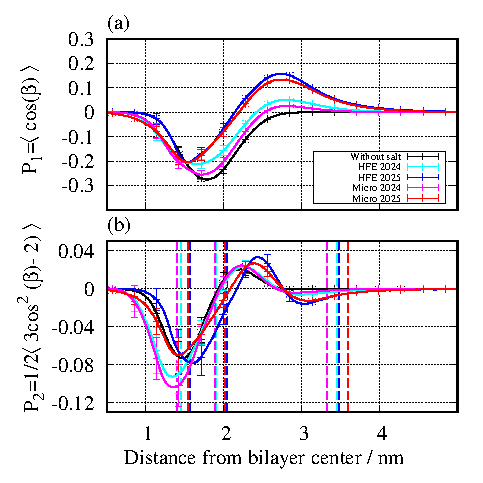
\includegraphics{figures/Figure_1.eps}
\end{figure}
The histogram of $P_2$ is used to calculate the \emph{hydration boundary} of the lipid bilayer system. The outermost
region of negative ordering is fitted to an exponential function, and the length scale of the exponential is used to find the location where $P_2$ is considered to be effectively zero. 
Lines to delimit these values are drawn on the plot in figure~\ref{fig:h2order}, and these positions are noted for each bilayer
in table~\ref{tab:struc}.
\begin{table}
{\tiny
    \caption{Bilayer structural parameters. The bilayer hydration boundary is defined as the position away from the bilayer center beyond which solvent is isotropic, and denotes 
        bulk solvent from bound solvent. The number of adsorbed charges in each adsorption mode are within the hydration boundary of the system, and are further classified by the degree
    of loss of hydration water -- steric adsorbed have lost no water, imperfect have lost at least one, and perfect have replaced all water oxygens for lipid oxygens. The bilayer thickness
\dhh{} is defined as the distance between the peaks in the electron density of the system, roughly localizing the phosphate groups. \dc{} is the thickness of the acyl-chain region of the bilayer,
and is measured as the distance between the Gibb's surfaces of the acyl-chain probability density. Lipid component volumes $V_{CH3}$ and $V_{\text{CH1/CH2}}$ are computed using the method
of Petrache \etal{}~\cite{petrache:1997}. $V_C$ is computed from the component volumes by multiplying by the number of these components in each acyl chain. 
$A_L=\frac{V_C}{D_C}$ is the two-dimensional area occupied per lipid on the bilayer surface. We note a correlation between simulations with larger numbers of adsorbed charges
and perturbation of the bilayer structure from that of the simulation without salt, especially in the bilayer \dc{}.}
    \label{tab:struc}
    \begin{tabularx}{\textwidth}{|X|X|X|X|X|X|}

        \hline                     & Without salt             &  \mg{ 2024} HFE     & \mg{ 2024} Micro    & \mg{ 2025} HFE    & \mg{ 2025} Micro \\\hline
    Hydration Boundary~(\AA)       & N/A                      &  34.5               & 33.3               & 34.8               & 35.9      \\\hline
    Perfectly Adsorbed Charges     & 0                        &  1.90               & 0.00               & 0.00               & 0.00      \\\hline
    Imperfectly Adsorbed Charges   & 0                        &  3.68               & 6.23               & 28.43              & 96.93     \\\hline
    Sterically Adsorbed Charges    & 0                        &  37.11              & 31.45              & 106.00             & 20.11     \\\hline
    $D_{HH}$~(\AA)                 & 37.57 $\pm$ 1.27         &  38.15 $\pm$ 1.20   & 37.75 $\pm$ 1.19   & 40.75 $\pm$ 0.92   & 40.26 $\pm$ 0.96\\\hline
%    $D_b$~(\AA)                    & 36.25 $\pm$ 0.47        & 43.01 $\pm$ 0.49   & 41.81 $\pm$ 0.52   & 46.24 $\pm$ 0.39   & 45.75 $\pm$ 0.42\\\hline
    $2D_C$~(\AA)                   & 26.98 $\pm$ 0.35         &  28.99 $\pm$ 0.31   & 28.08 $\pm$ 0.40   & 31.45 $\pm$ 0.29   & 30.84 $\pm$ 0.29\\\hline
    $V_{\text{CH1/CH2}}$~(\AA$^3$) & 26.33 $\pm$ 0.05         &  26.21 $\pm$ 0.05   & 26.33 $\pm$ 0.05   & 26.22 $\pm$ 0.04   & 26.12 $\pm$ 0.04\\\hline
    $V_{CH3}$~(\AA$^3$)            & 54.97 $\pm$ 0.39         &  54.77 $\pm$ 0.39   & 54.98 $\pm$ 0.40   & 54.74 $\pm$ 0.24   & 55.19 $\pm$ 0.26\\\hline
%    $V_H$~(\AA$^3$)                & 323.30 $\pm$ 0.82       & 323.95 $\pm$ 1.26  & 327.85 $\pm$ 1.10  & 283.55 $\pm$ 0.77  & 296.16 $\pm$ 0.67\\\hline
    $V_C$~(\AA$^3$)                & 899.72 $\pm$ 1.01        &  895.85 $\pm$ 1.05  & 899.83 $\pm$ 1.06  & 895.94 $\pm$ 0.95  & 894.00 $\pm$ 1.11\\\hline
%    $V_L$~(\AA$^3$)                & 1223.01 $\pm$ 0.82      & 1219.80 $\pm$ 1.24 & 1227.68 $\pm$ 1.24 & 1179.49 $\pm$ 1.02 & 1190.16 $\pm$ 1.07\\\hline
    $A_L=\frac{V_C}{D_C}$          & 66.71 $\pm$ 0.89         &  61.80 $\pm$ 0.66   & 64.10 $\pm$ 0.92   & 56.97 $\pm$ 0.54   & 57.98 $\pm$ 0.57\\\hline
    \end{tabularx}
}
\end{table}
\section{\mg Adsorption Behavior}
We classify any ion within the hydration boundary as at least sterically adsorbed, with further distinction -- steric, imperfect, or perfect -- based on how much dehydration the ion undergoes when approaching the bilayer center. A \emph{perfectly} adsorbed ion has lost all waters in its first hydration shell and an  \emph{imperfectly} adsorbed ion
has lost at least one water from its first coordination shell. 
{\emph{Sterically} adsorbed} waters have their first shell of waters intact, but 
they are spatially located within the \emph{hydration boundary} of the lipid bilayer. To evaluate this, we define a cutoff to the first hydration shell,
computed from radial distribution functions. The cutoff used for \mg{} in all systems is 3.3~\AA, which captures the first peak for \mg{} and lipid oxygens, water, and \cl{}. 
We compute the nearest oxygens (lipid phosphate, glycerol, ester fragment, \cl{}, or water) within these
cutoffs of cations across the simulation system, and generate a histogram averaged over slices and then over the last 150 ns of simulation time. This histogram is shown in 
figure~\ref{fig:ioncoordination}.
\begin{figure}[H]
    \caption{Coordination partners of \mg{}. We note that while the Micro water with the 2024 parameters do result in some dehydration 
        of the \mg{} in the headgroup region of the bilayer, both 2024 parameters yield nearly no dehydration of \mg{} at any location in the simulation box. The 2025 HFE parameters
        still largely do not dehydrate, but the 2025 Micro parameters do result in loss of 1-2 waters from the \mg{} coordination shell within the headgroup region. 
        We see substantial interaction with the headgroup phosphate oxygens, and no significant interaction with the glycerol or ester linkage oxygens. We also note the increased interaction with \cl{} in the 
    simulations using the 2025 parameters compared to both simulations with the 2024 parameters. The number of first shell \cl{} remains below one per ion in any simulation.}
\label{fig:ioncoordination}
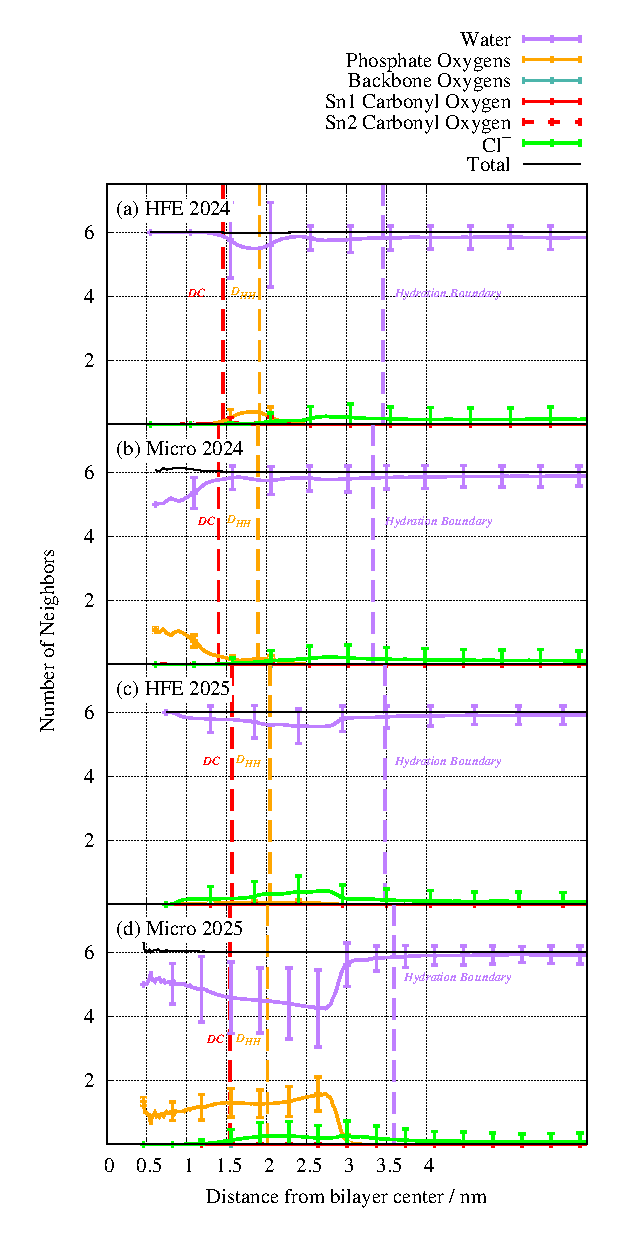
\includegraphics[height=0.5\textheight]{../figures/Figure_2.eps}
\end{figure}
We note that the \mg{ 2024} parameters result in very little dehydration of ions, throughout the simulation box. The 2025 parameters result in loss of 1-2 waters as the ion approaches the bilayer center, with the \mg{ 2025} Micro parameters resulting in the greatest degree of dehydration among parameter sets.
The \mg{ 2025} HFE parameters result in some loss of first shell water, but no replacement in the first shell with lipid oxygens. There are a significant number of \mg{}-\cl{} pairs, where a single \cl{} replaces a water
in the first shell of \mg{} as the ion moves into the lipid-occupied region of the bilayer. If these ions do not otherwise lose water for lipid parts, 
they are counted as \emph{sterically} adsorbed.

The \mg{ 2025} Micro parameters appear to have a preference for direct interaction with the phosphate group oxygens when dehydrated, and none of the \mg{} parameters studied result in significant direct interaction with the ester fragment and glycerol oxygens. There are also far fewer pairs with \cl{} under this parameter set.
Fractions of ions in each adsorption mode have been computed by counting the number of ions in each frame within the hydration boundary, 
and the number of those that have lost one water, or all of their waters. We compute averages over the last 150ns, and then 
fractions of the total adsorbed ions present in each mode. These values are shown in figure~\ref{fig:adfrac}, alongside the fraction of ions adsorbed vs the fraction remaining in bulk solvent. 
\begin{figure}[H]
    \caption{ (a) Distribution of \mg{} ions in different membrane adsorption modes. \mg{} are first classified into those in bulk and those adsorbed in membranes. 
        Among those adsorbed in membrane, \mg{} are 
        further classified into those that are perfectly, imperfectly and sterically adsorbed. 
        We note that compared to the 2024 models, the 2025 models result in increased membrane adsorption, 
        and among the adsorbed \mg{}, the 2025 models result in increased direct coordination with lipid headgroups. Next to the plot, we show examples of \mg{} in the \emph{steric} (b) and \emph{imperfect} (c) 
        adsorption modes from our simulations. The \emph{perfect} adsorption mode does not occur in a significant frequency in \mg{}, so an example is not included. We note that
    in this example of the \emph{steric} adsorption mode (b) there is a \cl{} (green) included in the hydration shell of the \mg{} ion (magenta). This is an example of a partial-ion
pair, which while having lost a water from the first-shell, it is not coordinating lipid components directly -- these are counted as sterically adsorbed.}
    \label{fig:adfrac}
    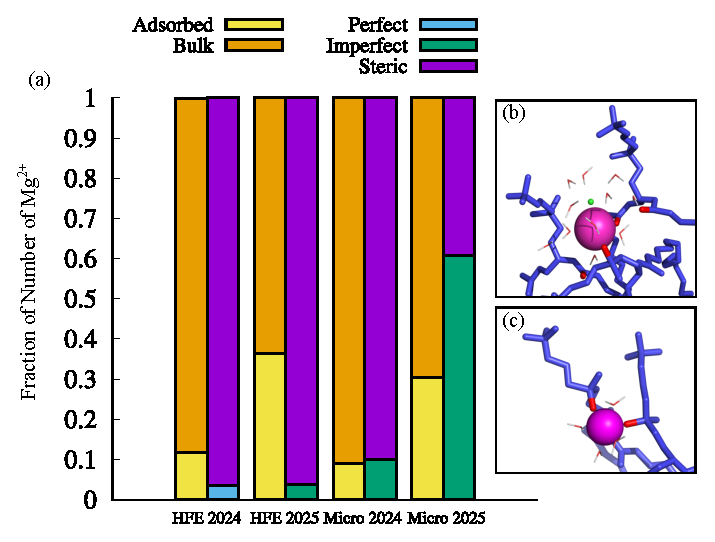
\includegraphics[height=0.5\textheight]{../figures/Figure_3.eps}
\end{figure}
The 2025 parameters result in significantly more adsorbed ions and as a result more adsorbed charges in both cases, with the most increased in the \mg{ 2025} HFE simulation.
We count the number of adsorbed charges in each adsorption mode by multiplying the number of ions in each mode by their charge; this would be 2 charges per \mg{}, and a \mg{} paired with a \cl{}
counts a single charge. 
These numbers can be seen in table~\ref{tab:struc} rows 2-4.
We also note an increase in imperfectly adsorbed ions in the \mg{ 2025} HFE simulation. However, the \mg{ 2025} Micro parameters result in ions shifting to the majority in the imperfect
adsorption mode from the steric mode seen in both 2024 simulations.
The \mg{ 2025} HFE parameters still remain with the largest fraction of ions in the steric adsorption mode. 
These differences in the distribution of adsorbed \mg{} ions -- particularly the rise in imperfect adsorption for \mg{ 2025} Micro -- 
raises the question of how such interactions reshape the membrane itself. We therefore turn to a structural analysis of the lipid bilayer 
to evaluate the consequences of these adsorption patterns.


\section{Bilayer Structure}
The effect of changes in ion adsorption on bilayer structure was assessed through several structural parameters. Electron densities were
computed using the \texttt{gmx density} tool included in the GROMACS software suite. Histograms were calculated in 1 ns chunks along the
bilayer normal (z-axis) and centered at zero using the position of minimum density, corresponding approximately to the bilayer midplane.
These histograms were then symmetrized about the center and averaged over the final 150 ns of each trajectory.

From the resulting profiles, we calculated the small-angle X-ray scattering (SAXS) form factor by subtracting the average water electron
density and applying a cosine transform. Electron density profiles and corresponding simulated SAXS form factors are shown in
Figure~\ref{fig:formfactors}.

\begin{figure}[H]
    \caption{SAXS form-factors and associated electron densities for \mg{} simulations. (a) \mg{ 2024} under both Micro
and HFE has little effect in changing the bilayer form-factor compared to that of the no-salt simulation, consistent with the available experimental results at lower ion concentrations. 
Conversely, both of the simulations with 2025 parameters result in significant thickening of the bilayer. 
This is also seen in the associated electron densities (b), where we see much taller peaks that are further apart in the \mg{ 2025} simulations
than that obtained from the 2024 simulations.}
    \label{fig:formfactors}
    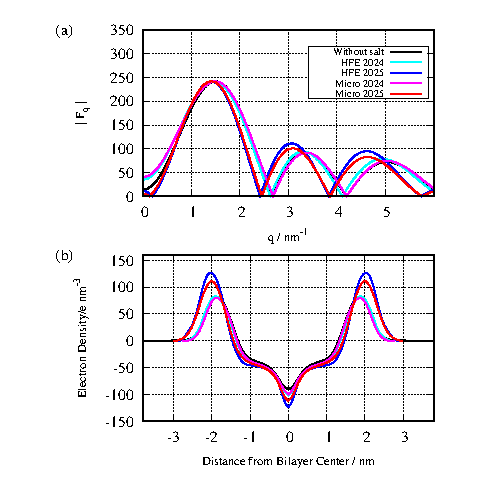
\includegraphics[height=0.5\textheight]{figures/Figure_4.eps}
\end{figure}
We note significant broadening of the bilayer peak-to-peak distance in the electron densities of the 2025 systems, compared to the 2024 systems. 
Additional structural parameters are computed from the various number density histograms of our simulations. Similarly to the electron densities, we use the gromacs GMX density tool to compute the number density histogram over 1ns chunks of our simulation. We then center these histograms using the centerpoint found from the electron
density at each 1ns chunk. 
These histograms are then symmetrized, and averaged over the last 150ns of simulation time. 
These can be seen for solvent and lipid headgroup components of in figure~\ref{fig:soldens}.
We note greater accumulation of \mg{} in the \mg{ 2025} simulations, with greater peak densities of cations in the headgroup regions, with the largest peak in the \mg{ 2025} HFE system. 

\begin{figure}[H]
    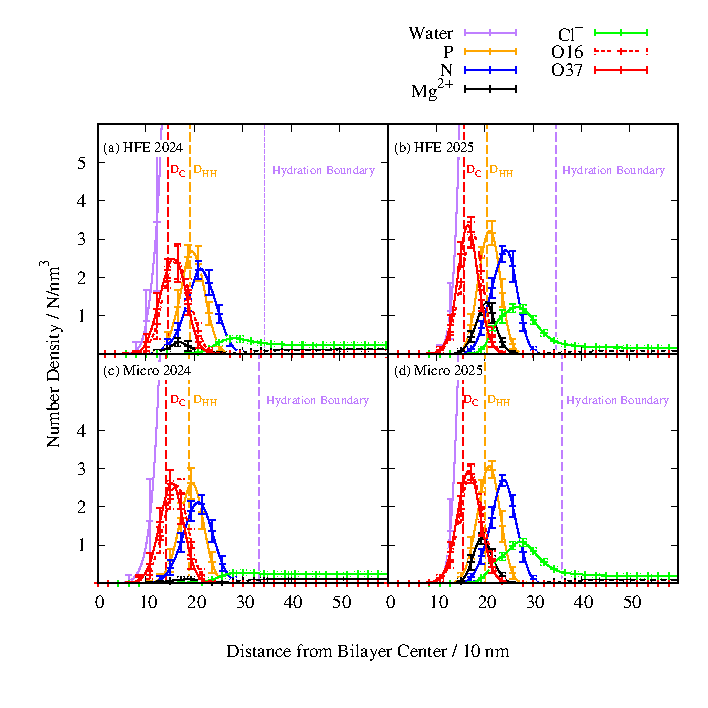
\includegraphics{figures/Figure_5.eps}
    \caption{Number density histograms of lipid headgroup components. Vertical lines denote the bilayer structural features such as the hydration boundary in purple, the \dhh{} in orange and the \dc{} in red. We note
    that within the hydration boundary of each system there is accumulation of ions -- anions accumulate near the trimethylammonium nitrogen and cations accumulate near the phosphate group. The \mg{ 2025} parameters
have a much larger accumulation of both ions in the headgroup region of the bilayer compared to the \mg{ 2024} systems.}
    \label{fig:soldens}
\end{figure}

The bilayer thickness \db{} and the acyl-chain region thickness \dc{} are computed as the distance between the Gibb's surfaces of the probability densities of solvent and the lipid acyl-chain carbons, respectively~\cite{fogarty:2015}. 
These are computed from the number densities of these species for each 1ns chunk of the simulation, and then averaged over the last 150ns of the simulation time.
The values for these are listed in table~\ref{tab:struc}. 
We also compute the lipid component volumes using the method of Petrache \etal{}~\cite{petrache:1997}. To do this, we partition the lipid number densities into 
headgroup and chains, with the headgroup consisting of any particles above the acyl chain ester fragment and the chains as just the acyl chain carbons. We partition the
chains into groups of CH2+CH1, and the terminal CH3 atoms. We optimize the following objective function to partition the volume in each histogram slice $z_j$ from the number densities to these groups:
\begin{equation}
    \Omega{(v_i)}=\sum^{\rho_s}_{z_j}\bigg(1-\sum^{N_{\text{groups}}}_{i=1}\big(\rho_i(z_j)(v_i)^2\bigg)\text{.}
\end{equation}
From this we obtain partial volumes for the groups $v_{\text{CH1\&CH2}}$, $v_{\text{CH3}}$, $v_{\text{Headgroup}}$. We equate the $V_{CH2}=v_{CH1\&CH2}$ as these densities have significant overlap, 
and thus the volumes cannot be separated. This, along with the $V_{\text{CH3}}=v_{\text{CH3}}$ can be seen in table~\ref{tab:struc}. These volumes multiplied by the number of each 
moiety in a lipid are used to compute \Vc. Finally, we compute the \al as the ratio $2\times{}V_c/2D_C$.

We note that in the systems with the smallest number of adsorbed charges in non-steric modes (perfect and imperfect) -- in this case the 2024-\mg parameters, show 
the smallest increase in \dc{}. The \mg{ 2025} systems have the greatest number of adsorbed charges in non-steric modes, 
and have the largest increase in \dc{} over the system simulated without salt. We note that
this trend is not followed necessarily in the \dhh{}, which is not a reliable measures of bilayer thickness due to the effect of headgroup tilt angle, and overlapping number densities of water
and salt in the headgroup region.
Together, we note that the systems with the greatest number of charges in the Langmuir-type (non-steric) modes correlate with an increase the 
bilayer thickness (figure~\ref{fig:chargeperlipid})
\begin{figure}[h!]
    \caption{Adsorbed charge per adsorption modality per lipid as a function of the lipid bilayer hydrocarbon thickness \dc{}. We compare both our results from this work, and our previous work with monovalent
        ions~\cite{saunders:2024}. There is a clear trend in the total number of adsorbed
        charges (i.e. any charges not in bulk solvent), where more charges results in a greater \dc{}. However, if one examines the sterically adsorbed charges, the trend is not as strong. This seems to indicate
    that the non-steric charges are most responsible for the pertubation of the bilayer thickness from that of the no-salt simulation shown as the blue region on the plot.}
    \label{fig:chargeperlipid}
    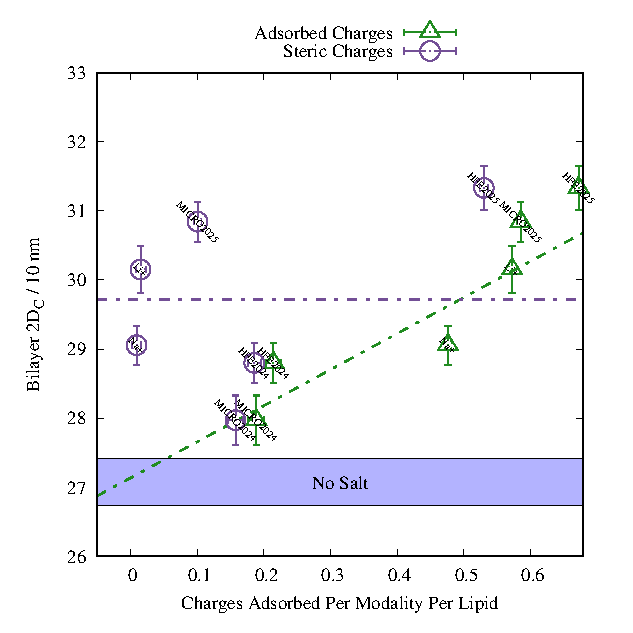
\includegraphics[height=0.5\textheight]{figures/Figure_6.eps}
\end{figure}
\section{Conclusions}
We have presented a comparison between
two \mg{} parameter sets developed by our
group, under two different water–ion
interaction models. The \mg{ 2024}
parameters, optimized using clusters of
ions and lipid-component ligands at
sub-full oxygen coordination of the
ion~\cite{saunders:2024}, predict steric
adsorption with negligible bilayer
thickening. By contrast, the \mg{ 2025}
parameters, optimized using fully
coordinated clusters by replacing the
missing ligand oxygens with
waters, similar to sets of target data used to improve parameters for \mg{-nucleotide} phosphate interactions~\cite{julian:2023:mg}, yield
significantly more ions in non-steric
adsorption modes, greater direct
coordination with lipid phosphates, and a
correlated increase in bilayer thickness.
Both parameter sets reproduce their
respective substitution energy targets,
but the choice of partially versus fully
coordinated clusters leads to divergent
predictions for bilayer behavior.
 This raises a fundamental question about the nature of
\mg{} adsorption, and potentially of
divalent ions in general. Both
water-separated and direct-interaction
adsorption modes have been described for
\mg{}–phosphate interactions in biological
molecules~\cite{grotz:thesis,micro,grotz:2021:optimized,
villaparams,dudev:2003,rulivsek:2003:outer,
porschke:1979:mode,bowman:2012,fingerhut:2021:contact},
and simulations with older ion models tend
to favor the water-separated
modes~\cite{grotz:thesis,micro,grotz:2021:optimized,
villaparams,puyo:2022:consistent}. With
sparse experimental data for lipid bilayers
at relevant salt concentrations, it is not
yet possible to judge between these models.
Thus, the two parameter sets serve as
complementary hypotheses and experimental
targets, highlighting that the critical open
question is not only which parameters best
reproduce bilayer structure, but also which
underlying reference chemistry most
faithfully represents \mg{–lipid}
interactions in the condensed phase.

\FloatBarrier
\section{Supporting Information}
The Supporting Information includes parameter bounds and active constraints for the
Lennard--Jones terms used in \mg--lipid interactions, comparative plots of
\mg--ligand cluster geometries optimized with quantum mechanical and molecular
mechanics methods, and references supporting the computational methodology.

\section{Acknowledgements}
Authors SV and MS acknowledge funding for this study was provided partly by the National Institute of Health RO1 GM147210
\bibliography{refs}
\newpage

\end{document}
